\documentclass[t,compress,mathserif,12pt,xcolor=dvipsnames]{beamer}
\setbeamertemplate{bibliography item}{\insertbiblabel}
\usepackage{etex}
\reserveinserts{28}
\definecolor{bleuUni}{RGB}{3, 184, 222}
\definecolor{marronUni}{RGB}{68, 58, 49}
\usecolortheme[named=bleuUni]{structure}
\usepackage[bars]{beamerthemetree} % Beamer theme v 2.2
\usepackage{multimedia}
\usepackage[utf8]{inputenc}
%\usepackage[frenchb]{babel}
\usepackage[T1]{fontenc}
\usepackage{kmath,kerkis}
\usepackage{xmpmulti}
%\usepackage{mathpazo}
%\usepackage[bitstream-charter]{mathdesign}
%\usepackage{lmodern}
\usepackage{booktabs}
\usepackage{multirow}
\usepackage{pgfplots}
\pgfplotsset{compat=newest}
\usepackage{tikz}
\usetikzlibrary{patterns, shapes, arrows}
\usepackage{mathtools}
\usepackage{listings}
\usepackage{eulervm}
\usepackage{pifont}% http://ctan.org/pkg/pifont
\newcommand{\cmark}{\ding{51}}%
\newcommand{\xmark}{\ding{55}}%
\usepackage{listings}
\usepackage{array}
\newcolumntype{L}[1]{>{\raggedright\let\newline\\\arraybackslash\hspace{0pt}}m{#1}}
\newcolumntype{C}[1]{>{\centering\let\newline\\\arraybackslash\hspace{0pt}}m{#1}}
\newcolumntype{R}[1]{>{\raggedleft\let\newline\\\arraybackslash\hspace{0pt}}m{#1}}

\lstset{
  language=C++,
  basicstyle=\tiny\ttfamily,
  numbers=left,
  numberstyle=\tiny\ttfamily,
  stepnumber=1,
  numbersep=5pt,
  backgroundcolor=\color{white},
  showspaces=false,
  showstringspaces=false,
  showtabs=false,
  frame=single,
  tabsize=2,
  captionpos=b,
  breaklines=true,
  breakatwhitespace=false,
  escapeinside={(*@}{@*)},
  identifierstyle=\ttfamily,
  keywordstyle=\color[rgb]{0,0,1},
  commentstyle=\color[rgb]{0.133,0.545,0.133},
  stringstyle=\color[rgb]{0.627,0.126,0.941},
  moredelim=[is][\underbar]{**}{**},
}

\lstdefinestyle{mycpp}
{
    language = C++,
    % numbers=left,
    % numbersep=0.3em,
    escapeinside={(*@}{@*)},
    tabsize=2,
    % basicstyle=\tiny\ttfamily,
    morekeywords = {constexpr,int8_t,int16_t,int32_t, size_t},
    % commentstyle=\color{comment-color},
}

\usepackage[backend=biber, style=ieee]{biblatex}
\addbibresource{bibli.bib}
\renewcommand\mkbibacro[1]{{\footnotesize\MakeUppercase{#1}}}

\mode<presentation>
\newcommand*\oldmacro{}%
\let\oldmacro\insertshorttitle%
\renewcommand*\insertshorttitle{%
 \oldmacro\hfill%
\insertframenumber\,/\,\inserttotalframenumber}
\setbeamertemplate{footline}[frame number]
\setbeamersize{text margin left=10pt,text margin right=10pt}
\setbeamerfont{frametitle}{size=\large}
\setbeamertemplate{frametitle}{ \nointerlineskip \begin{beamercolorbox}[wd=\paperwidth,ht=2.2ex,dp=0.5ex,left]{frametitle} \hspace*{3.1ex}\strut\bfseries\color{bleuUni!15!white}\insertframetitle\strut\par \end{beamercolorbox}}

\setbeamertemplate{bibliography item}{\insertbiblabel}
  \definecolor{bluecite}{HTML}{009DE0}


\makeatletter
\def\beamer@andinst{\\[0.1em]}
\makeatother
%~~~~~~~~~~~~~~~~~~~~~~~~~~~~~~~~~~~~~~~~~~~~~~~~~~~~~~~~~~~
%\setbeamercovered{higly dynamic}
\usetheme{Ilmenau} % Beamer theme v 3.0
%\useoutertheme[subsection=true]{smoothbars}%Beamer Outer Theme-circles on top
\setbeamercolor{section in head/foot}{bg=marronUni}

\useinnertheme{circles} %rectangle bullet points instead of circle ones
\usepackage{beamerthemebars}
\setbeamercolor{navigation symbols dimmed}{fg=red!80!black}
\setbeamercolor{navigation symbols}{fg=red!80!black}
\setbeamertemplate{navigation symbols}{}%remove navigation symbols
%~~~~~~~~~~~~~~~~~~~~~~~~~~~~~~~~~~~~~~~~~~~~~~~~~~~~~~~~~~~~~~~~~~~~~
\title{\textbf{Candidature au poste de \\ Maître de conférence en électronique numérique}}
%\subtitle{algorithms et arhitecture}\hspace{10.7cm}
\author[Mathieu Léonardon\hspace{3.01cm}\url{https://mathieuleonardon.com}\hspace{1.0cm}{mathieu.leonardon@ims-bordeaux.fr}]{\Large{Mathieu Léonardon}\vspace{-0.5cm}}
\titlegraphic{\includegraphics[height=2cm]{logos/IMT_Atlantique_logo.png}}
\date{14 Mai 2019}
\input{colors}

\definecolor{dgreen}{rgb}{0.,0.6,0.}
\definecolor{milano}{rgb}{0.458824, 0.050980, 0.058824}
\definecolor{bahama}{rgb}{0.066667, 0.298039, 0.443137}
\definecolor{blupres}{RGB}{0, 157, 224}
\definecolor{redpres}{RGB}{204, 0, 0}

\newcommand\blfootnote[1]{%
  \begingroup
  \renewcommand\thefootnote{}\footnote{#1}%
  \addtocounter{footnote}{-1}%
  \endgroup
}



\newcommand{\RED} [1]{\textcolor{Paired-5}{\textbf{#1}}}
\newcommand{\ORANGE} [1]{\textcolor{orange}{\textbf{#1}}}
\newcommand{\GREEN} [1]{\textcolor{Paired-3}{\textbf{#1}}}
\newcommand{\BLUE} [1]{\textcolor{Paired-1}{\textbf{#1}}}

\newcommand{\MILANO} [1]{\textcolor{milano}{#1}}
\newcommand{\BAHAMA} [1]{\textcolor{bahama}{#1}}

\usepackage{textpos}
%\usepackage{stmaryrd}
\usepackage{amsbsy}
\usepackage{makecell}
%\usepackage{fourier-orns}
% \usepackage{tikz}
% \usetikzlibrary{patterns, shapes, arrows, shapes.multipart}

\usepackage{etoolbox}
\AtBeginSection[]
{
	% \ifnumcomp{\value{section}}{=}{1}{}{
\begin{frame}[t]{Plan}
\centering
\tableofcontents[
  currentsection,
  currentsubsection,
  sectionstyle=show/shaded,
  subsectionstyle=show/show/shaded,
]
\end{frame}
% }
}
% \AtBeginSubsection[]
% {
% 	\begin{frame}[t]{}
% \tableofcontents[
% currentsection,
% sectionstyle=show/show,
% subsectionstyle=show/shaded/hide
% ]
% 	\end{frame}
% }


% \defbeamertemplate*{title page}{customized}[1][]
% {
%   \usebeamerfont{title}\inserttitle\par
%   \usebeamerfont{subtitle}\usebeamercolor[fg]{subtitle}\insertsubtitle\par
%   \bigskip
%   \usebeamerfont{author}\insertauthor\par
%   \usebeamerfont{institute}\insertinstitute\par
%   \usebeamerfont{date}\insertdate\par
%   \usebeamercolor[fg]{titlegraphic}\inserttitlegraphic
% }

\bibliography{bibli}


% \includeonly{part2}

\begin{document}

\begin{frame}[t]
\titlepage
\end{frame}

\section{Cursus}
\subsection{Formation d'ingénieur}
\begin{frame}[t]{Formation d'ingénieur - Cours}
  \begin{minipage}[t][5.0cm][t]{\textwidth}
    \begin{columns}[T]
      \begin{column}{0.63\textwidth}
        \begin{itemize}
          \item<+-> Enseirb-Matmeca (Bordeaux)
          \item<+-> "Systèmes Electroniques Embarqués"
          \begin{itemize}
            \item<+-> FPGA et ASIC (Langage VHDL)
            \item<+-> Architecture des ordinateurs
            \item<+-> Programmation uC
            \item<+-> OS embarqués
          \end{itemize}
        \end{itemize}
      \end{column}
      \begin{column}{0.04\textwidth}

      \end{column}
      \begin{column}{0.33\textwidth}
        \only<1->{\centering\includegraphics[width=0.5\textwidth]{fig/UBx}\\ \vspace{0.5cm}}
        \only<3->{\includegraphics[width=0.5\textwidth]{fig/fpga}\\ \vspace{0.5cm}}
        \only<4->{\includegraphics[width=\textwidth]{fig/stages}}
      \end{column}
    \end{columns}
  \end{minipage}
  \begin{figure}[htp]
    \centering
    \only<1-2>{\includegraphics[width=\textwidth]{fig/frise1}}
    \only<3-4>{\includegraphics[width=\textwidth]{fig/frise2}}
    \only<5->{\includegraphics[width=\textwidth]{fig/frise3}}
  \end{figure}
\end{frame}
\begin{frame}[t]{Formation d'ingénieur - Apprentissage}
  \begin{minipage}[t][5.0cm][t]{\textwidth}
    \begin{columns}[T]
      \begin{column}{0.63\textwidth}
        \begin{itemize}
          \item<+-> Entreprise WorldCast Systems
          \item<+-> Broadcast
          \item<+-> \'Equipe R\&D émetteurs FM
          \begin{itemize}
            \item<+-> Conception de cartes électroniques
            \item<+-> Programmation de uC
            \item<+-> Projet : IHM
          \end{itemize}
        \end{itemize}
      \end{column}
      \begin{column}{0.04\textwidth}

      \end{column}
      \begin{column}{0.33\textwidth}
        \only<1->{\includegraphics[width=\textwidth]{fig/worldcast}\\}
        \only<3-5>{\vspace{0.8cm}\includegraphics[width=\textwidth]{fig/helios}\\}
        \only<6->{\includegraphics[width=\textwidth]{fig/engi}}
      \end{column}
    \end{columns}
  \end{minipage}
  \begin{figure}[htp]
    \centering
    \only<1-5>{\includegraphics[width=\textwidth]{fig/frise3}}
    \only<6>{\includegraphics[width=\textwidth]{fig/frise4}}
  \end{figure}


\end{frame}

\subsection{Doctorat}
\begin{frame}[t]{Décodage de Codes Polaires}
  \begin{minipage}[t][5.0cm][t]{\textwidth}
  \vspace{1cm}
  \centering
  Décodage de codes polaires sur des architectures programmables
    % \begin{columns}
      % \begin{column}{0.63\textwidth}
        % \vspace{-30pt}
          % \begin{itemize}
            % \item Décodage de codes polaires sur des architectures programmables
            % \item Cotutelle Canada - France
          % \end{itemize}
      % \end{column}
      % \begin{column}{0.04\textwidth}

    %   \end{column}
    %   \begin{column}{0.33\textwidth}
    %     \only<+->{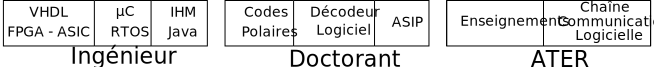
\includegraphics[width=\textwidth]{fig/frise}\\ \vspace{0.5cm}}
    %     \only<+->{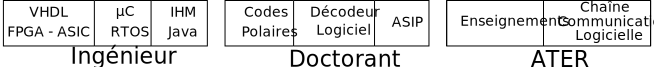
\includegraphics[width=\textwidth]{fig/frise}\\ \vspace{0.5cm}}
    %     \only<+->{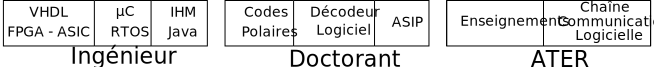
\includegraphics[width=\textwidth]{fig/frise}}
    %   \end{column}
    % \end{columns}
  \end{minipage}
  \begin{figure}[htp]
    \centering
    \includegraphics[width=\textwidth]{fig/frise5}
  \end{figure}
\end{frame}

\begin{frame}[t]{Implémentation logicielle SC Liste}
  \begin{minipage}[t][5.0cm][t]{\textwidth}
    \begin{columns}[T]
      \begin{column}{0.63\textwidth}
        \begin{itemize}
          \item<+-> Décodeurs logiciels - x86\_64 \& ARM
          \item<+-> Parallélisation
          \begin{itemize}
            \item<2-> SIMD, multithreads, multinodes
          \end{itemize}
          \item<+-> Implémentation flexible et générique
          \item<+-> Adaptatif le plus rapide à ce jour
          \item<+-> Intégré avec le projet AFF3CT
          \begin{itemize}
            \item<5-> \url{https://aff3ct.github.io}
          \end{itemize}
        \end{itemize}
      \end{column}
      \begin{column}{0.04\textwidth}

      \end{column}
      \begin{column}{0.33\textwidth}
        \only<1->{\includegraphics[width=\textwidth]{fig/throughput}\\ \vspace{0.5cm}}
        \only<5->{\includegraphics[width=\textwidth]{fig/chain_ink}}
      \end{column}
    \end{columns}
  \end{minipage}
    \begin{figure}[htp]
    \centering
    \includegraphics[width=\textwidth]{fig/frise6}
  \end{figure}
\end{frame}

\begin{frame}[t]{Architectures ASIP pour le décodage de codes polaires}
  \begin{minipage}[t][5.0cm][t]{\textwidth}
    \begin{columns}[T]
      \begin{column}{0.56\textwidth}
        \begin{itemize}
          \item<+-> Architecture 1 - Tensilica
          \begin{itemize}
            \item<1-> Collaboration Pierre Langlois (Polytechnique Montréal)
          \end{itemize}
          \vspace{1.5cm}
          \item<+-> Architecture 2 - TTA
          \begin{itemize}
            \item<2-> Collaboration Pekka Jääskeläinen (TUT)
          \end{itemize}
        \end{itemize}
      \end{column}
      \begin{column}{0.04\textwidth}

      \end{column}
      \begin{column}{0.40\textwidth}
        \only<1->{\includegraphics[width=\textwidth]{fig/full_tensilica}\\ \vspace{0.5cm}}
        \only<2->{\includegraphics[width=\textwidth]{fig/tta_base}}
      \end{column}
    \end{columns}
  \end{minipage}
  \begin{figure}[htp]
    \centering
    \includegraphics[width=\textwidth]{fig/frise7}
  \end{figure}


\end{frame}

\begin{frame}[c]{Publications}

  \begin{enumerate}
\renewcommand{\section}[2]{} % Trick to avoid references section

    \renewcommand*{\bibfont}{\scriptsize}
    \nocite{leonardon_fast_2017,leonardon_custom_2018,ghaffari_improving_2017,leonardon_tta_2018,Ghaffari2018,cassagne_fast_2017,cassagne_gdr_2017,leonardon_custom_2018}
    \vfill
    \item<+-> Implémentation logicielle de l'algorithme  SCL
    \scriptsize{\printbibliography[keyword={fast-scl}]}
    \vfill
    \item<+-> Spécialisation d'un processeur Tensilica
    \scriptsize{\printbibliography[keyword={tensilica}]}
    \vfill
    \item<+-> Conception d'un processeur de type TTA
    \scriptsize{\printbibliography[keyword={tta}]}
    \vfill
  \end{enumerate}

\end{frame}

\begin{frame}[c]{Publications}

  \begin{enumerate}
\renewcommand{\section}[2]{} % Trick to avoid references section

    \renewcommand*{\bibfont}{\scriptsize}
    \nocite{leonardon_fast_2017,leonardon_custom_2018,ghaffari_improving_2017,leonardon_tta_2018,Ghaffari2018,cassagne_fast_2017,cassagne_gdr_2017}
    \vfill
    \item<+-> Implémentation du décodeur SCMA
    \printbibliography[keyword={ghaffari}]
    \vfill
    \item<+-> Contribution au projet AFF3CT
    \printbibliography[keyword={aff3ct}]
    \vfill
  \end{enumerate}

\end{frame}


\subsection{Poste ATER}
\begin{frame}[t]{Enseignement}
  \begin{minipage}[t][5.0cm][t]{\textwidth}
    \vspace{-0.5cm}
    \begin{itemize}
      \item<+-> \'Electronique numérique
      \begin{itemize}
        \item<1-> Projet de conception en \'electronique (50 HETD)
        \item<1-> Architecture reconfigurable (20 HETD)
        \item<1-> \'Electronique Num\'erique (25 HETD)
        \item<1-> Logique combinatoire et logique s\'equentielle (32 HETD)
      \end{itemize}
      \vspace{0.3cm}
      \item<+-> Informatique
      \begin{itemize}
        \item<2-> Projet micro-processeur (36 HETD)
        \item<2-> Architecture des ordinateurs (16 HETD)
        \item<2-> Projet micro-informatique (42 HETD)
        \item<2-> Programmation objet. Langage C++ (15 HETD)
      \end{itemize}
    \end{itemize}

  \end{minipage}
  \begin{figure}[htp]
    \centering
    \includegraphics[width=\textwidth]{fig/frise8}
  \end{figure}
\end{frame}

\begin{frame}[t]{Travaux}
 \begin{minipage}[t][5.0cm][t]{\textwidth}
    \begin{columns}[T]
      \begin{column}{0.63\textwidth}
          \begin{itemize}
            \item Projet industriel (Airbus Defense \& Space)
            \begin{itemize}
              \item Radio logicielle
              \item Communications satellitaires
            \end{itemize}
          \end{itemize}
      \end{column}
      \begin{column}{0.04\textwidth}

      \end{column}
      \begin{column}{0.33\textwidth}
        \only<+->{\includegraphics[width=\textwidth]{fig/chaine_airbus}}
      \end{column}
    \end{columns}
  \end{minipage}
  \begin{figure}[htp]
    \centering
    \includegraphics[width=\textwidth]{fig/frise9}
  \end{figure}
\end{frame}

\section{Intégration}
\subsection{Enseignement}
\begin{frame}[t]{Enseignements de première année}
  \begin{minipage}[t][5.0cm][t]{\textwidth}
    \begin{columns}[T]
      \begin{column}{0.63\textwidth}
          \begin{itemize}
            \item<+-> Opérationnel sur l'enseignement d'électronique numérique,
            \item<+-> Apte à encadrer les différents projets (FAIRE, SAR, CODEV).
          \end{itemize}
      \end{column}
      \begin{column}{0.04\textwidth}

      \end{column}
      \begin{column}{0.33\textwidth}
        \only{\includegraphics[width=\textwidth]{fig/loto}}
      \end{column}
    \end{columns}
  \end{minipage}
  \begin{figure}[htp]
    \centering
    \only<1>{\includegraphics[width=\textwidth]{fig/frise10}}
    \only<2>{\includegraphics[width=\textwidth]{fig/frise11}}
  \end{figure}


\end{frame}

\begin{frame}[t]{TAF Systèmes Embarqués Hétérogènes}
  \begin{minipage}[t][5.0cm][t]{\textwidth}
  \centering
  \vspace{0.8cm}
  «La double compétence logicielle et matérielle, indissociable des systèmes embarqués, est très recherchée.»

  \end{minipage}
  \begin{figure}[htp]
    \centering
    \includegraphics[width=\textwidth]{fig/frise12}
  \end{figure}
\end{frame}

\begin{frame}[t]{UE Coeurs}
  \begin{minipage}[t][5.0cm][t]{\textwidth}
    \begin{columns}[T]
      \begin{column}{0.63\textwidth}
        \begin{itemize}
            \item<+-> UEC1 : Circuits intégrés numériques et analogiques
            \item<+-> UEC2 : Méthodologies - de l’algorithme à la puce
            \item<+-> UEC3 : Systèmes embarqués
        \end{itemize}
      \end{column}
      \begin{column}{0.04\textwidth}

      \end{column}
      \begin{column}{0.33\textwidth}
        \only<1>{\includegraphics[width=.9\textwidth]{fig/UEC1}}
        \only<2>{\includegraphics[width=.9\textwidth]{fig/UEC2}}
        \only<3>{\includegraphics[width=.9\textwidth]{fig/UEC3}}
      \end{column}
    \end{columns}
  \end{minipage}
  \begin{figure}[htp]
    \centering
    \only<1>{\includegraphics[width=\textwidth]{fig/frise13}}
    \only<2>{\includegraphics[width=\textwidth]{fig/frise14}}
    \only<3>{\includegraphics[width=\textwidth]{fig/frise15}}
  \end{figure}


\end{frame}

\begin{frame}[t]{UE \'Electives}
  \begin{minipage}[t][5.0cm][t]{\textwidth}
    \begin{columns}[T]
      \begin{column}{0.63\textwidth}
        \begin{itemize}
            \item<+-> UEE : Conception haut niveau de circuits
            \item<+-> UEE : IA Intro \& IA Optimisation
            \item<+-> UEE : Workshop à Grenoble - recherche et industrie des micro et nanotechnologies
            \item<+-> UEE : Calcul parallèle
        \end{itemize}
      \end{column}
      \begin{column}{0.04\textwidth}

      \end{column}
      \begin{column}{0.33\textwidth}
        \only<1>{\includegraphics[width=.9\textwidth]{fig/UEE1}}
        \only<2>{\includegraphics[width=.9\textwidth]{fig/UEE3}}
        \only<3>{\includegraphics[width=.9\textwidth]{fig/UEE4}}
        \only<4>{\includegraphics[width=.9\textwidth]{fig/UEE2}}
      \end{column}
    \end{columns}
  \end{minipage}
  \begin{figure}[htp]
    \centering
    \only<1>{\includegraphics[width=\textwidth]{fig/frise16}}
    \only<2>{\includegraphics[width=\textwidth]{fig/frise17}}
    \only<3>{\includegraphics[width=\textwidth]{fig/frise17}}
    \only<4>{\includegraphics[width=\textwidth]{fig/frise18}}
  \end{figure}



\end{frame}


\begin{frame}[t]{TAF CoOC}
  \begin{minipage}[t][5.0cm][t]{\textwidth}
        \begin{itemize}
          \item<+-> Conception centrée utilisateur
          \item<+-> Prototypage rapide et développement agile
          \item<+-> L'objet dans son environnement
          \item<+-> Projet fil rouge
          \begin{itemize}
            \item<+-> Maquettage
            \item<+-> \'Etude des utilisateurs
            \item<+-> Rédaction cahier des charges
          \end{itemize}
        \end{itemize}
  \end{minipage}
  \begin{figure}[htp]
    \centering
    \includegraphics[width=\textwidth]{fig/frise19}
  \end{figure}


\end{frame}
\subsection{Recherche}
\begin{frame}[t]{Codes Polaires}
  \begin{minipage}[t][5.0cm][t]{\textwidth}
    \begin{columns}[T]
      \begin{column}{0.63\textwidth}
        \vspace{-0.5cm}
        \begin{itemize}
          \item<+-> Expertise développée au cours de ma thèse
          \item<+-> Axes de recherche possibles
          \begin{itemize}
            \item<+-> Implémentations matérielles flexibles
            \item<+-> Implémentations logicielles hautes performance
            \item<+-> Algorithmes à sortie souple
            \item<+-> Nouvelles constructions : multinoyaux, assymétriques
          \end{itemize}
        \end{itemize}
      \end{column}
      \begin{column}{0.04\textwidth}

      \end{column}
      \begin{column}{0.33\textwidth}
        \only<1->{\includegraphics[width=\textwidth]{fig/sc}\\ \vspace{0.5cm}}
        \only<3->{\includegraphics[width=\textwidth]{fig/ilp-1}}
      \end{column}
    \end{columns}
  \end{minipage}
  \begin{figure}[htp]
    \centering
    \includegraphics[width=\textwidth]{fig/frise20}
  \end{figure}
\end{frame}

\begin{frame}[t]{Simulation haut débit de chaînes de communications}
  \begin{minipage}[t][5.0cm][t]{\textwidth}
    \begin{columns}[T]
      \begin{column}{0.63\textwidth}
        \begin{itemize}
          \item<+-> Expertise dans les simulations haut débits (AFF3CT)
          \vspace{0.3cm}
          \item<+-> Réalisation de démonstrateurs (USRP)
          \vspace{0.5cm}
          \item<+-> Modulation (FBMC/OQAM)
          \item<3-> Entrelaceurs de turbo-codes
          \item<3-> Modulation codée
          \item<3-> ...
        \end{itemize}
      \end{column}
      \begin{column}{0.04\textwidth}
      \end{column}
      \begin{column}{0.33\textwidth}
        \centering
        \only<1->{\includegraphics[width=0.3\textwidth]{fig/aff3ct}\\ \vspace{0.2cm}}
        \only<2->{\includegraphics[width=\textwidth]{fig/usrp}}
      \end{column}
    \end{columns}
  \end{minipage}
  \begin{figure}[htp]
    \centering
    \includegraphics[width=\textwidth]{fig/frise21}
  \end{figure}
\end{frame}

\begin{frame}[t]{ASIP}
  \begin{minipage}[t][5.0cm][t]{\textwidth}
    \begin{itemize}
      \item<+-> Nombreux travaux sur architectures ASIP (DecASIP)
      \item<+-> Intégration : compétent sur les différents langages ASIP (incl. LISA + Synopsys)
      \item<+-> Intégration : intérêt des architectures TTA
    \end{itemize}
    \only<1>{
      \vspace{-2cm}
      \begin{enumerate}
        \renewcommand{\section}[2]{} % Trick to avoid references section
        \renewcommand*{\bibfont}{\tiny}
        \nocite{6579576,7155493,6654620,6683963,6571888,7041196}
        \printbibliography[keyword={asip-amer}]
      \end{enumerate}
    }
    \only<3>{
      \centering
      \includegraphics[width=0.6\textwidth]{fig/ilp-1}
    }
  \end{minipage}
  \begin{figure}[htp]
    \centering
    \includegraphics[width=\textwidth]{fig/frise22}
  \end{figure}
\end{frame}

\begin{frame}[t]{Collaborations internationales}
  \begin{minipage}[t][5.0cm][t]{\textwidth}
    \begin{columns}[T]
      \begin{column}{0.63\textwidth}
        \small{
          \begin{itemize}
            \item<+-> Thèse en cotutelle avec Polytechnique Montréal
            \begin{itemize}
            \item<1-> Yvon Savaria, Directeur de thèse
            \item<1-> Pierre Langlois, Co-auteur
            \end{itemize}
            \vspace{0.8cm}
            \item<+-> Thibaud Tonnellier, McGill University (Canada), Co-auteur
          \end{itemize}
        }
      \end{column}
      \begin{column}{0.04\textwidth}
      \end{column}
      \begin{column}{0.33\textwidth}
      \centering
        \only<1->{\vspace{0.6cm}\includegraphics[width=0.5\textwidth]{fig/poly}\\\vspace{1.6cm} }
        \only<2->{\includegraphics[width=0.5\textwidth]{fig/mcgill}\\}
      \end{column}
    \end{columns}
  \end{minipage}
  \begin{figure}[htp]
    \centering
    \includegraphics[width=\textwidth]{fig/frise23}
  \end{figure}
\end{frame}


\begin{frame}[t]{Collaborations internationales}
  \begin{minipage}[t][5.0cm][t]{\textwidth}
    \begin{columns}[T]
      \begin{column}{0.63\textwidth}
        \small{
          \begin{itemize}
            \item<+-> Pekka Jääskelainen, TUT (Finlande), Co-auteur
            \item<+-> Vyacheslav Klymentiev, Saint Petersburg Electrotechnical University (Russie), AFF3CT
            \item<2-> Peter Trifonov, Saint Petersburg Polytechnic University (Russie), AFF3CT
            \item<2-> Chen Shuang, Tsinghua University (Chine), AFF3CT
          \end{itemize}
        }
      \end{column}
      \begin{column}{0.04\textwidth}
      \end{column}
      \begin{column}{0.33\textwidth}
      \centering
        \only<1->{\includegraphics[width=1\textwidth]{fig/tampere}\\\vspace{-0.1cm}}
        \only<2->{\includegraphics[width=0.26\textwidth]{fig/etu}\\\vspace{0.5cm}}
        \only<2->{\includegraphics[width=0.5\textwidth]{fig/polysp}\vspace{-0.2cm}\\}
        \only<2->{\includegraphics[width=0.7\textwidth]{fig/tsinghua}}

      \end{column}
    \end{columns}
  \end{minipage}
  \begin{figure}[htp]
    \centering
    \includegraphics[width=\textwidth]{fig/frise23}
  \end{figure}
\end{frame}
\end{document}

